\section{An Overview of OpenMP's Evolution}
\label{sec:evolve}

OpenMP is a living language that reflects the needs of its many users. 
As hardware capabilities and the range of supported algorithms have 
grown, the complexity of the specification has also expanded. 
Figure~\ref{omppcount} lists the number of pages of the versions of 
the specification (not including front matter, appendices or indices).   
The initial OpenMP specification (OpenMP Version 1.0 for Fortran) was 
40 pages long. The latest specification (OpenMP 4.5 for Fortran, 
C and C++) is 303 pages long.

Figure~\ref{omppcount} also details the evolution of language support.
Prior to the release of version 2.5 in 2005, each OpenMP specification 
was specialized to a particular language (i.e., to Fortran or to C and 
C++). This division simplified writing the text of the specification, 
but also created difficulties. First, most of the people working on the 
Fortran specifications also worked on the C/C++ specifications. Thus, the 
evolution of the API was hampered since we could not run the two 
language committees in parallel. Thus, updates to the specification 
were produced slowly relative to the amount of new material in them.
For example, OpenMP 2.0 for C/C++ (50 pages) was released almost 4 years 
after OpenMP 1.0 for C/C++ (45 pages) despite the relatively simple 
extensions that it included. 

Not only was the progress of the API slower due to the separate 
specifications, the separation also allowed the API to have subtle 
differences across the languages. The process of merging the separate
APIs for the languages into a single  specification was a much larger 
undertaking than any of us expected. That process required us to recast 
OpenMP's core abstractions much more carefully so they would apply across 
the languages. The resulting OpenMP version 2.5 specification (117 pages)
took three years to create despite adding few new capabilities.

Following the merger of the specifications and the growth in the popularity
of the API, as evidenced by the expanding membership of the OpenMP ARB,
the pace of the evolution of OpenMP has increased. Today, OpenMP is no 
longer a simple API for which its full breadth can be learned in less 
than a day. Nonetheless, the core features of the version 1.0 specifications
remain and the goal of backwards copatibility has largely been achieved.

The OpenMP version 3.0 API specification (151 pages) added task-based 
parallelism. This addition supports irregular parallelism, unlike the 
loop-based constructs of the previous specifications. OpenMP 3.0 also
provided much more control over the existing support for structured
parallelism. OpenMP version 3.1 (160 pages) extended the support for 
structured parallelism, for example, by asdding straightforward control
of the number of threads used at each level of nested parallelism. 
OpenMP 3.1 also further refined tasking support. In general, the 
continued evolution of OpenMP has advanced the original features 
while also expanding the types of parallel algorithms that the 
specifcation supports.

The OpenMP version 4.0 API specification (248 pages) added support for 
accelerator-based systems through its device constructs. Echoing the API's 
original purpose, OpenMP 4.0 also standardized directives for SIMD 
parallelism, which had become widely supported by many compilers but 
with subtly different semantics. OpenMP 4.5 (303 pages) added many 
refinements to those addition and elsewhere. As we later discuss in 
detail, OpenMP 5.0 will support mechanisms to control data placement in
complex, multi-level memory systems. It will also include support for
first-party and third-party tools as well as the customary major 
extensions for the types of parallelism already supported by OpenMP.

In evolving the OpenMP API, we have added features that address 
non-uniform memory architectures, more complex concurrency control, 
irregular algorithms, accelerators, and much more. The specification 
has not grown due to a lack of discipline in its designers. Instead,
its growth reflects user demands for new features and how hardware 
has changed. In that light, a 7.5X increase in size over the course 
of almost 20 years is not surprising.

\begin{figure}
  \centering
  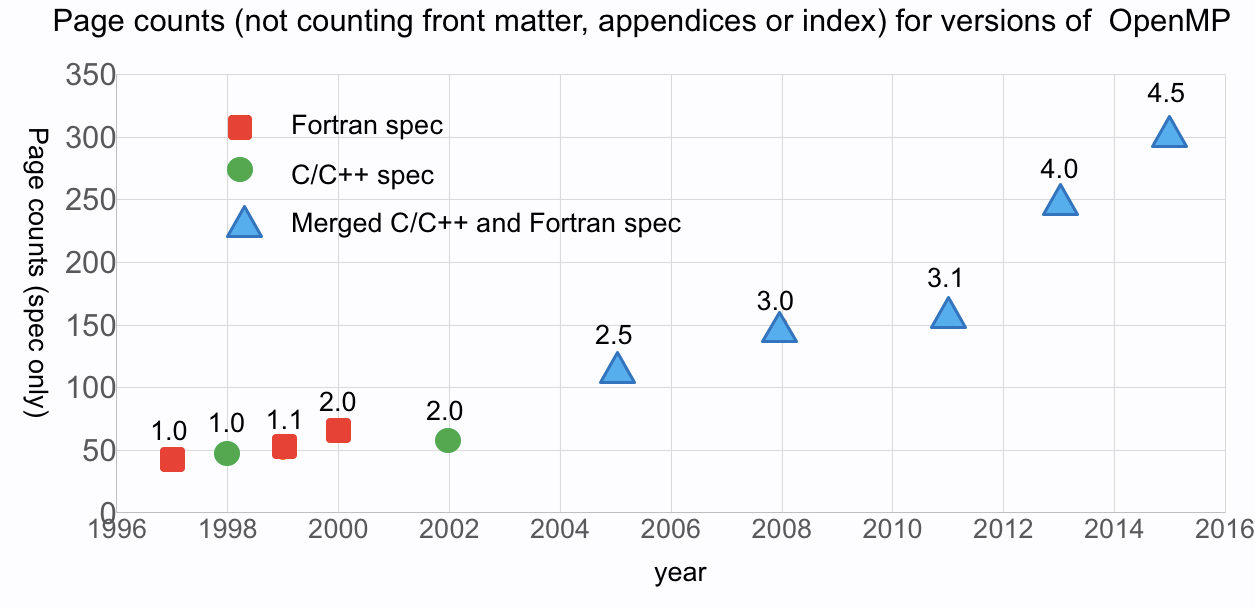
\includegraphics[width=3.4in]{pics/opcounts.png}
  \caption{OpenMP specification release dates, page counts and language bindings.}
  \label{omppcount}
\end{figure}


